\documentclass[12pt,onecolumn,a4paper,fleqn]{article}
\usepackage[top=1in, bottom=1in, left=0.75in, right=0.75in]{geometry}
\usepackage{epsfig,graphicx,amsthm,amsmath}
\usepackage[table,xcdraw,svgnames]{xcolor}
\usepackage{setspace}
\usepackage{mathtools}
\usepackage{fancyhdr}
\usepackage{sidecap}
\usepackage{caption}
\usepackage{subcaption}
\usepackage{tikz}
\usepackage{pgfplots}
\usetikzlibrary{decorations.pathreplacing}
\usepackage{relsize}
\usepackage{color,xcolor}
\usepackage[framed,numbered]{matlab-prettifier}
\usepackage{float}
\usepackage{enumerate}
\usepackage{booktabs}
\usepackage{wrapfig}
\usepackage{datetime}
\usepackage{xepersian}


\settextfont[Path=fonts/,BoldFont={ZarBd.ttf},BoldFeatures={Scale=0.9}]{BZar.ttf}

%\DeclarePairedDelimiter\ceil{\lceil}{\rceil}
%\DeclarePairedDelimiter\floor{\lfloor}{\rfloor}

%\definecolor{vgreen}{RGB}{104,180,104}
%\definecolor{vblue}{RGB}{49,49,255}
%\definecolor{vorange}{RGB}{255,143,102}


% title page template
\newcommand{\heading}[2]
{
	\begin{center}
		{\huge
			\textbf{
				به نام خدا\\
			}
		}
		
		\vspace*{1.5cm}
		
\includegraphics[scale=0.9]{source/sharif_logo.png}\\
		\vspace*{0.5cm}
		{\Large
			\textbf{
				دانشگاه صنعتی شریف\\
				\vspace*{0.25cm}
				دانشکده مهندسی کامپیوتر\\
			}
		}
		\vspace*{3cm}
		{\huge
			\textbf{
				آزمایشگاه معماری کامپیوتر\\
				\vspace*{0.75cm}
			}
		}
		
		{\Large
			\textbf{
				#1:\\
				#2\\
			}
		}
		
		\noindent\rule[1ex]{\linewidth}{1pt}\\
		\vspace*{0.5cm}
		\begin{table}[H]
			\centering
			\begin{tabular}{|c|c|}
				\hline
				\multicolumn{2}{|c|}{\textbf{اطلاعات تیم}}
				\\ \hline
				\textbf{نام اعضا} & \textbf{شماره دانشجویی}
				\\ \hline
				متین داغیانی & 98106456
				\\ \hline
				بردیا محمدی & 98171104
				\\ \hline
				محمدجواد هزاره & 98101074
				\\ \hline 
			\end{tabular}
		\end{table}
		{\Large				
			\vspace*{0.75cm}
			\textbf{
				پاییز 1400
			}}		
	\end{center}
}

\pagestyle{fancy}
\fancyhf{}
\rhead{\textbf{آزمایشگاه معماری کامپیوتر}}
%%--------------------[should change]---------------------
\chead{\textbf{گزارش آزمایش اول}}
%%--------------------[should change]---------------------
\lhead{\textbf{\nouppercase{\rightmark}}}
\cfoot{({\thepage})}
\renewcommand{\headrulewidth}{1pt}
\renewcommand{\footrulewidth}{1pt}
\renewcommand{\sectionmark}[1]{\markright{#1}}
\renewcommand{\subsectionmark}[1]{\markright{#1}}
%\newdateformat{monthyeardate}{%
%	\monthname[\THEMONTH], \THEYEAR}

\onehalfspacing
\begin{document}
	%%% title pages
	\large
	\begin{titlepage}
		\heading{آزمایش دوم}{ضرب‌کننده ممیز ثابت}
		\thispagestyle{empty}
	\end{titlepage}	
	\pagebreak
	
	%%% contents page
	\tableofcontents
	\thispagestyle{empty}
	\pagebreak
	
	%%% main document
	\section{هدف آزمایش}
	در این آزمایش هدف پیاده‌سازی مدار ضرب‌کننده دو عدد باینری ممیز ثابت بود. از آن‌جایی که ضرب دو عدد ممیز ثابت تفاوتی با ضرب دو عدد عادی ندارد و صرفا کافیست مکان ممیز را در انتها لحاظ کنیم، طراحی یک مدار ضرب کننده چهاربیتی خواسته‌ی ما را برآورده می‌کند.
	
	برای ضرب دو عدد باینری نیز از الگوریتم \lr{Add \& Shift} استفاده شده است که یک الگوریتم ترتیبی است. در این الگوریتم در هر مرحله با بررسی کردن بیت اول ضرب‌کننده، تصمیم گرفته می‌شود که ضرب‌شونده را به حاصل اضافه کنیم یا خیر. سپس ضرب‌کننده را یک واحد به سمت راست شیفت داده تا بیت بعدی آن مورد بررسی قرار گیرد، هم‌چنین ضرب‌شونده نیز یک واحد به سمت چپ شیفت داده می‌شود چرا که مرتبه‌ی بیتی که قرار است در آن ضرب شود، یک واحد افزایش پیدا کرده است.
	
	بنابراین برای طراحی مدار نیاز به ماژول‌های شیفت‌دهنده به سمت چپ، شیفت‌دهنده به سمت راست و یک جمع‌کننده هشت بیتی نیاز بوده که جزئیات طراحی این ماژول‌ها در بخش بعدی آمده است. در شکل
	\ref{fig:circuit_diag}
	نیز نمای کلی مدار طراحی شده آمده است که سیگنال‌های ورودی آن، شامل ضرب‌کننده و ضرب‌شونده به ترتیب با \lr{p} و \lr{q} نشان داده شده‌اند. سیگنال ورودی \lr{start} برای شروع کار مدار آمده است و خروجی در هشت بیت \lr{sum} نمایش داده شده که با یک شدن سیگنال \lr{end}، خروجی مدار آماده شده است.
	\begin{figure}[H]
		\centering
		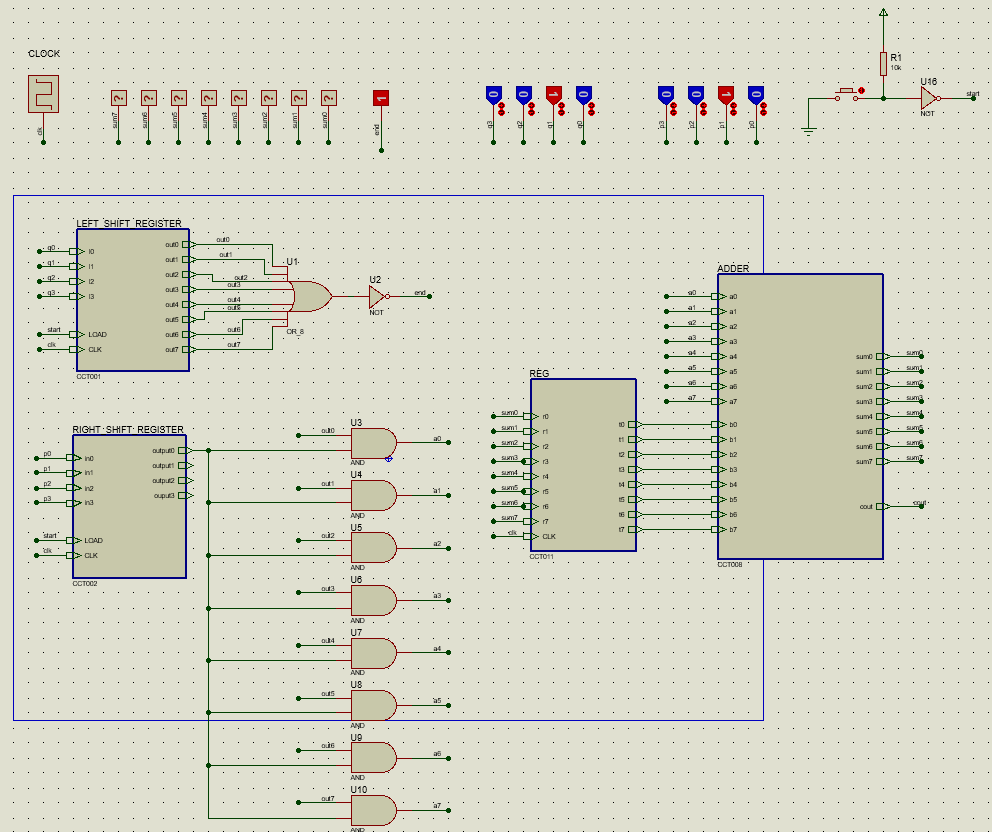
\includegraphics[width=0.75\textwidth]{source/circuit_diagram.png}
		\caption{نمای کلی مدار ضرب‌کننده}
		\label{fig:circuit_diag}
	\end{figure}
	\section{مراحل طراحی و پیاده‌سازی مدار}
	همانطور که در بخش قبل گفته شد، مدار مورد نظر از سه ماژول اصلی شیفت‌دهنده به سمت راست، شیفت‌دهنده به سمت چپ و جمع‌کننده هشت‌بیتی تشکیل شده است. هم‌چنین ماژول \lr{REG} ماژول کمکی بوده و برای جلوگیری از شلوغ شدن نمای اصلی مدار اضافه شده است. در ادامه به بررسی طراحی هر یک از این ماژول‌ها می‌پردازیم:
	\subsection{ماژول شیفت‌دهنده به سمت راست}
	\begin{wrapfigure}{l}{0.18\textwidth}
		\centering
		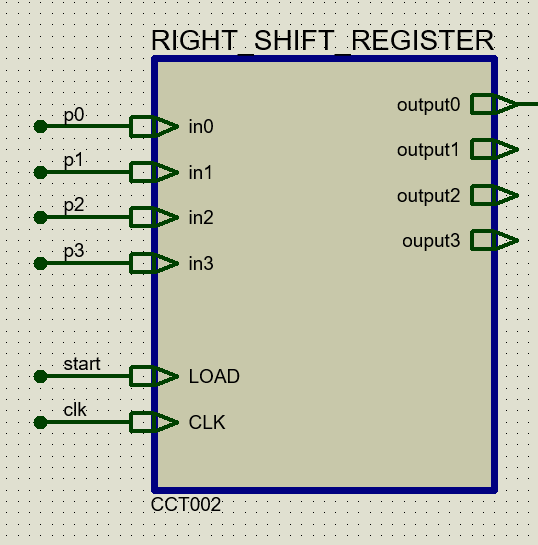
\includegraphics[width=0.17\textwidth]{source/rshiftreg.png}
		\caption{ورودی‌ها و خروجی‌های ماژول شیفت‌دهنده به سمت راست}
		\label{fig:rshiftreg}
	\end{wrapfigure}
همانطور که گفته شد این مدار برای شیفت دادن ضرب‌کننده در هر مرحله مورد استفاده قرار می‌گیرد. ورودی‌ها و خروجی‌های آن را در شکل \ref{fig:rshiftreg} می‌توان دید.

	طراحی داخلی این ماژول نیز به کمک فلیپ‌فلاپ‌های نوع \lr{D} صورت گرفته که خروجی هر یک به صورت سریال به فلیپ‌فلاپ بعدی داده شده تا عملیات شیفت با آمدن کلاک صورت بگیرد. طراحی داخلی این ماژول را در شکل \ref{fig:rshift_inner} می‌توان مشاهده کرد.
	\begin{figure}[H]
		\centering
		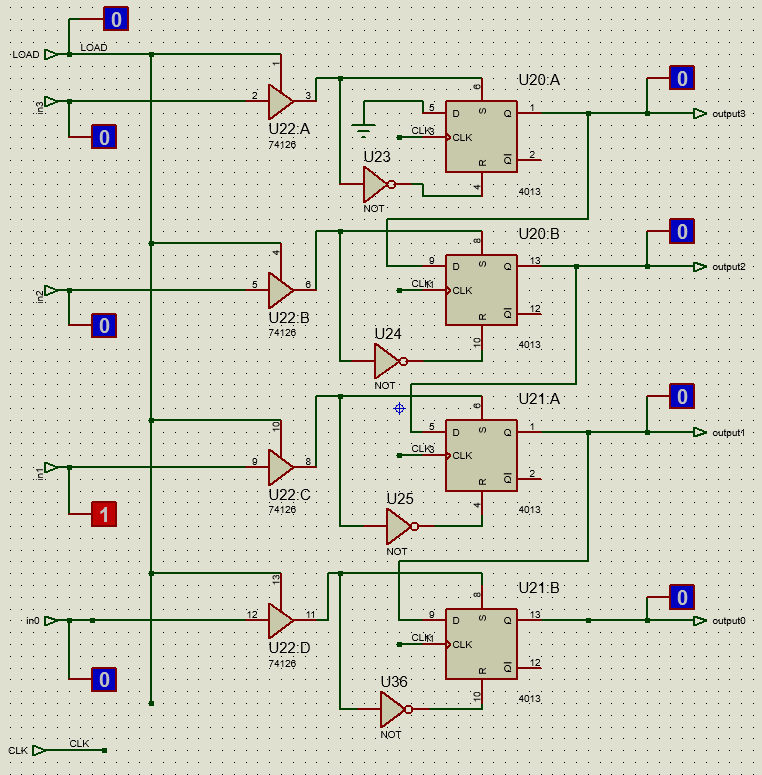
\includegraphics[width=0.5\textwidth]{source/rshift_inner.png}
		\caption{طراحی داخلی ماژول شیفت‌دهنده به سمت راست}
		\label{fig:rshift_inner}
	\end{figure}
	\noindent
	$\;\triangleleft$
	همانطور که در الگوریتم \lr{Add \& Shift} توضیح داده شد، از بیت اول مقدار شیفت داده شده‌ی ضرب‌کننده برای این منظور که ضرب‌شونده را به حاصل اضافه کنیم یا خیر استفاده می‌شود، بنابراین بیت اول خروجی این ماژول را با بیت‌های ضرب‌شونده \lr{And} می‌کنیم تا خواسته‌ی ما برآورده شود.
	\begin{figure}[H]
		\centering
		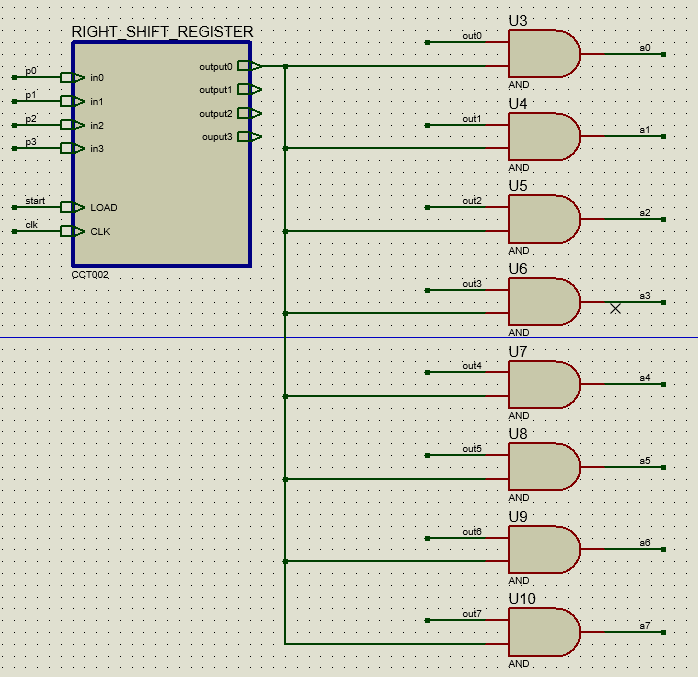
\includegraphics[width=0.5\textwidth]{source/decidetoadd.png}
		\caption{تصمیم‌گیری برای اضافه کردن ضرب‌شونده}
		\label{fig:decidetoadd}
	\end{figure}
	\subsection{ماژول شیفت‌دهنده به سمت چپ}
	از این ماژول برای شیفت دادن ضرب‌شونده به سمت چپ استفاده می‌شود. رابط این ماژول را در شکل \ref{fig:lshiftreg} می‌توان دید.
	\begin{figure}[H]
		\centering
		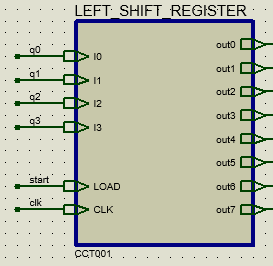
\includegraphics[width=0.5\textwidth]{source/lshiftreg.png}
		\caption{ماژول شیفت‌دهنده به سمت چپ}
		\label{fig:lshiftreg}
	\end{figure}
در طراحی داخلی این مدار نیز از فلیپ‌فلاپ‌های نوع \lr{D} استفاده شده که مشابه ماژول قبلی خروجی هر فلیپ‌فلاپ به ورودی فلیپ‌فلاپ قبلی متصل شده تا عملیت شیفت به چپ صورت بگیرد. طراحی داخلی این ماژول را نیز می‌توان در شکل \ref{fig:lshiftreg_inner} مشاهده کرد.
	\begin{figure}[H]
		\centering
		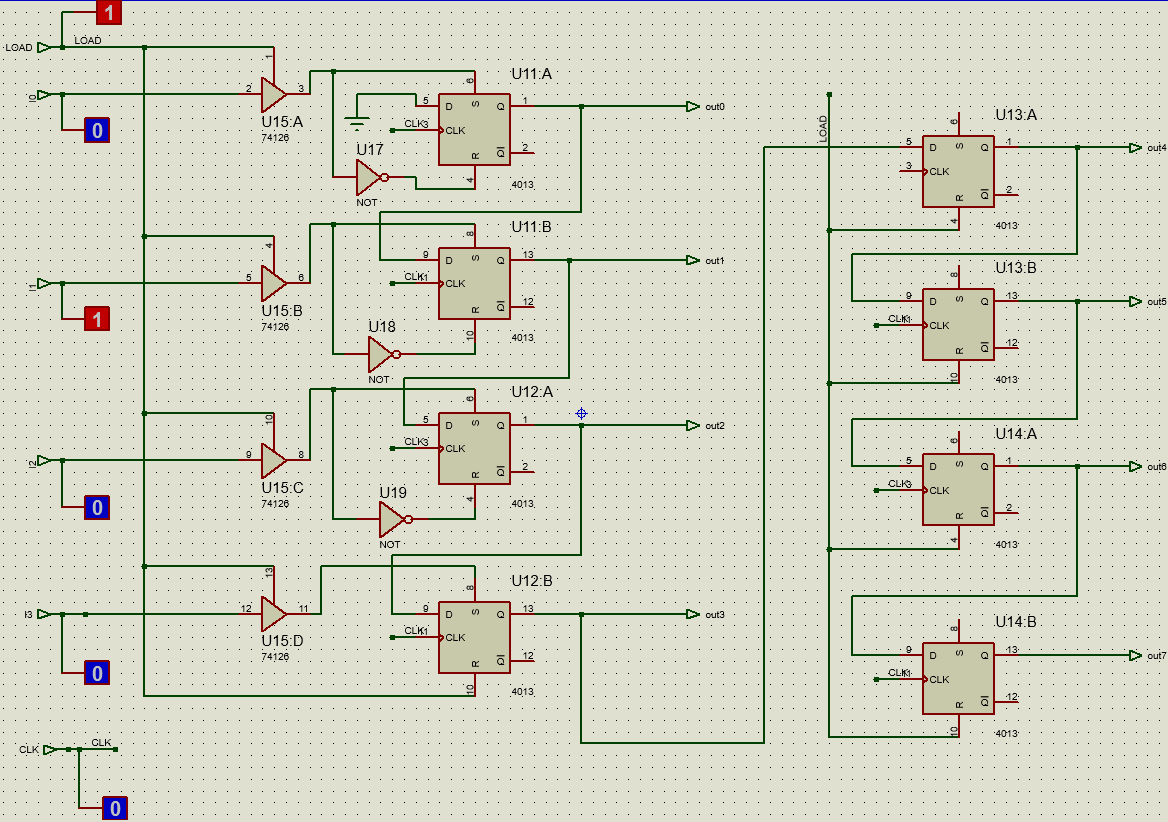
\includegraphics[width=0.5\textwidth]{source/lshiftreg_inner.png}
		\caption{طراحی داخلی ماژول شیفت‌دهنده به سمت چپ}
		\label{fig:lshiftreg_inner}
	\end{figure}
	\noindent
	$\;\triangleleft$
	از آن‌جایی که شیفت به سمت چپ با اضافه شدن صفر به سمت راست عدد به وجود می‌آید، می‌توان با صفر شدن همه‌ی بیت‌های مقدار حاصل از شیفت، به این موضوع پی برد که آیا الگوریتم به پایان رسیده است یا خیر. بنابراین از همین موضوع برای مشخص کردن سیگنال خروحی \lr{end} استفاده شده است. مدار این قسمت در شکل \ref{fig:end_signal} آورده شده است.
	\begin{figure}[H]
		\centering
		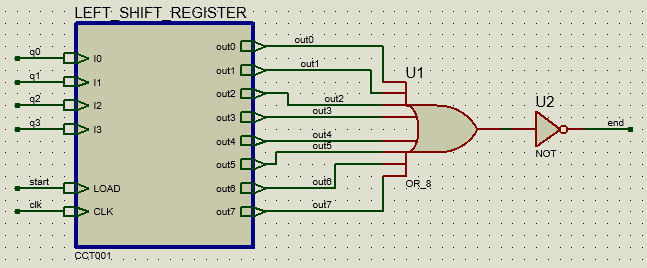
\includegraphics[width=0.5\textwidth]{source/end_signal.png}
		\caption{مشخص کردن مقدار سیگنال خروجی \lr{end}}
		\label{fig:end_signal}
	\end{figure}
	\subsection{ماژول جمع‌کننده}
	این ماژول وظیفه جمع کردن مقدار حاصل تا این لحظه، با ضرب‌شونده را داراست. در واقع مقدار ضرب‌شونده در سیگال‌های $a_i$ به این ماژول می‌رسد که این سیگنال‌ها همان  \lr{and} شده‌ی بیت‌های ضرب‌شونده با بیت اول ضرب‌کننده هستند. رابط این ماژول در شکل آمده است.
	\begin{figure}[H]
		\centering
		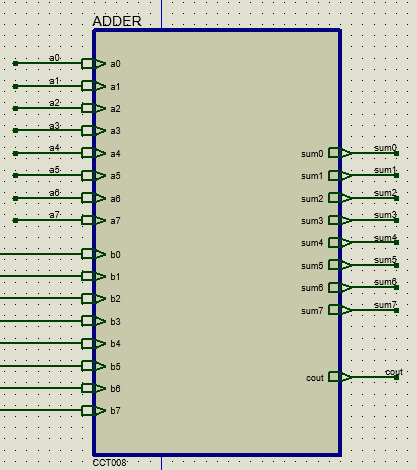
\includegraphics[width=0.5\textwidth]{source/adder.png}
		\caption{ماژول جمع‌کننده}
		\label{fig:adder}
	\end{figure}

	طراحی داخلی این جمع‌کننده نیز با استفاده از هشت \lr{Full Adder} صورت گرفته که طراحی داخلی این ماژول و ماژول \lr{Full Adder} را در شکل \ref{fig:adder_inner} می‌توان دید.
	\begin{figure}[H]
		\begin{subfigure}{0.5\textwidth}
			\centering
			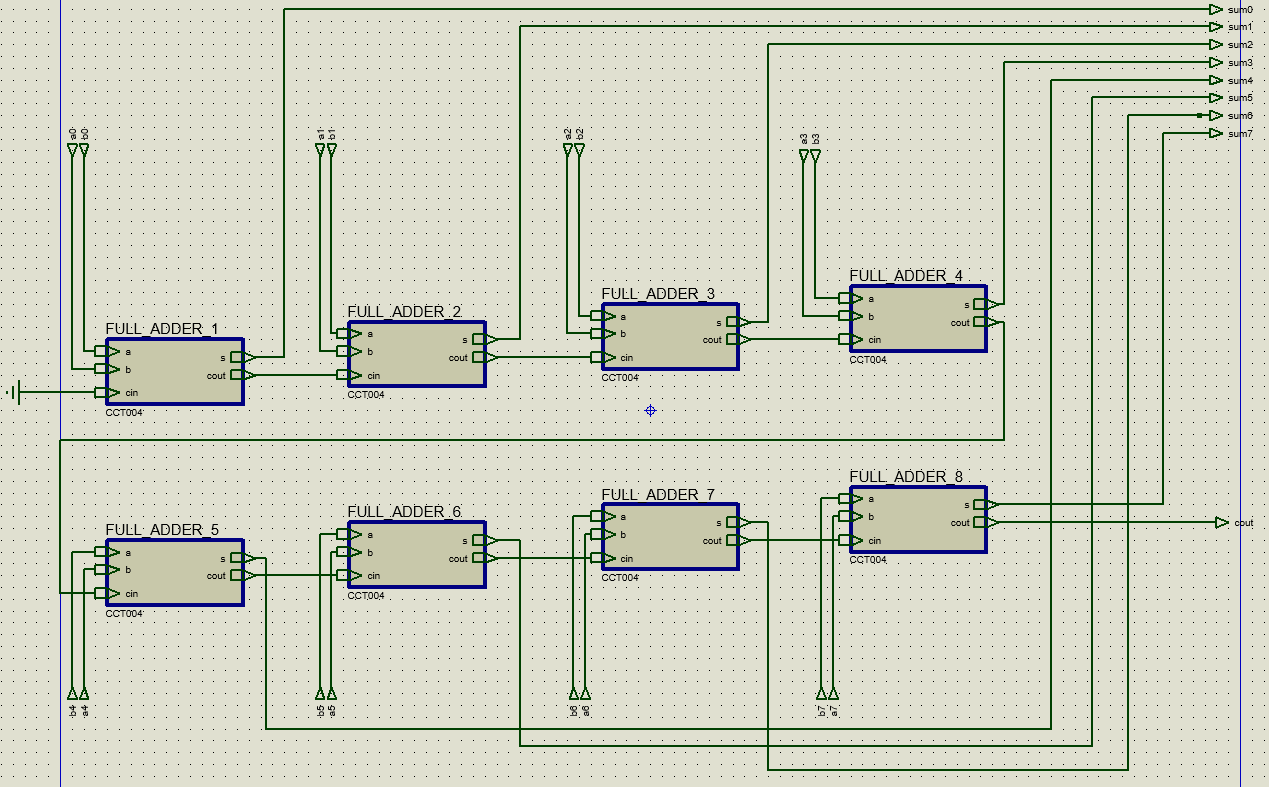
\includegraphics[width=\textwidth]{source/adder_inner.png}
			\caption{طراحی داخلی ماژول جمع‌کننده}
		\end{subfigure}
		\hfill
		\begin{subfigure}{0.4\textwidth}
			\centering
			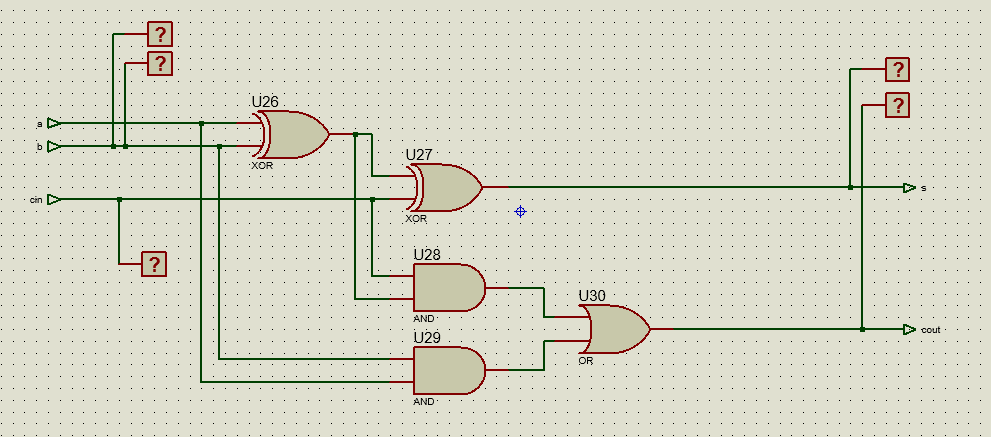
\includegraphics[width=\textwidth]{source/fulladder_inner.png}
			\caption{طراحی داخلی ماژول \lr{Full Adder}}
		\end{subfigure}
		\caption{طراحی داخلی \lr{Adder} و \lr{FullAdder}}
		\label{fig:adder_inner}
	\end{figure}
	\subsection{ماژول ‌\lr{REG}}
	همانطور که گفته شد این ماژول به عنوان رجیستر برای نگه‌داری مقدار حاصل ضرب در هر مرحله استفاده می‌شود. خروجی‌های این ماژول به ماژول جمع‌کننده داده شده تا مقدار حاصل ضرب آپدیت شود. ورودی‌ و خروجی‌های این ماژول در شکل \ref{fig:register} آورده شده است.
	\begin{figure}[H]
		\centering
		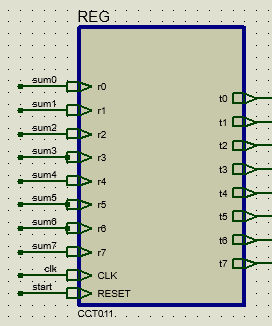
\includegraphics[width=0.4\textwidth]{source/register.png}
		\caption{ماژول \lr{REG}}
		\label{fig:register}
	\end{figure}
	در مدار داخلی آن نیز از هشت فلیپ‌فلاپ نوع \lr{D} استفاده شده است که طراحی آن را در شکل \ref{fig:register_inner} می‌توان دید.
	\begin{figure}[H]
		\centering
		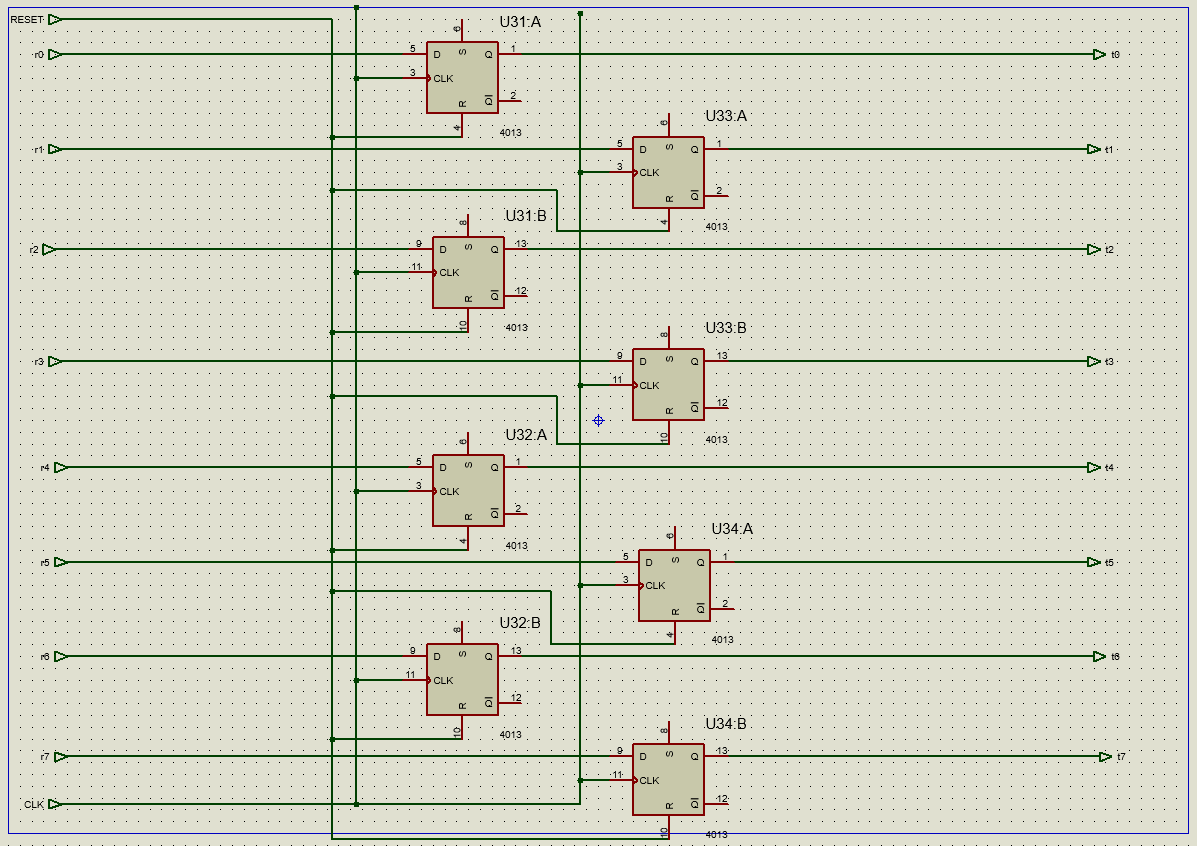
\includegraphics[width=0.5\textwidth]{source/register_inner.png}
		\caption{طراحی داخلی ماژول \lr{REG}}
		\label{fig:register_inner}
	\end{figure}
	\newpage
	\section{تست مدار}
	برای تست کارکرد مدار نیز چند نمونه ورودی داده شده و حاصل‌ضرب آن‌ها توسط مدار محاسبه شده است. نمونه‌ای از تست‌ها را در شکل‌های زیر می‌توان دید.
	\begin{figure}[H]
		\centering
		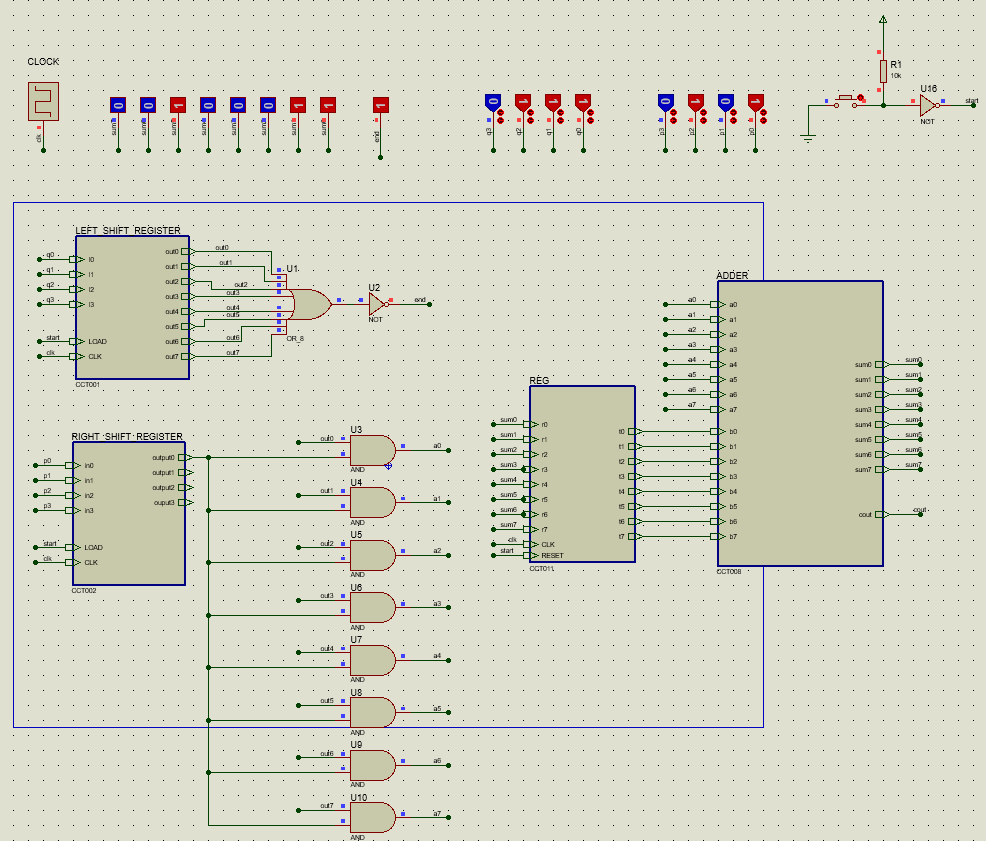
\includegraphics[width=0.8\textwidth]{source/test1.png}
		\caption{$7 \times 5 = 35$}
		\vspace*{5mm}
		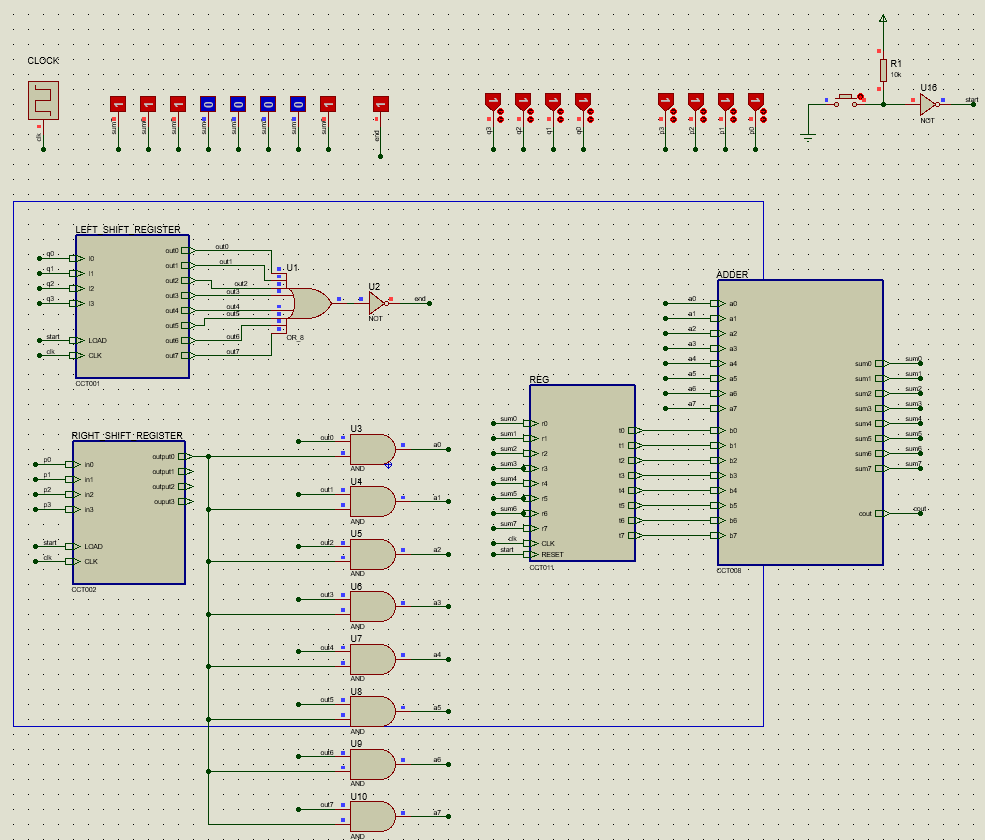
\includegraphics[width=0.8\textwidth]{source/test2.png}
		\caption{$15 \times 15 = 225$}
		\vspace*{5mm}
		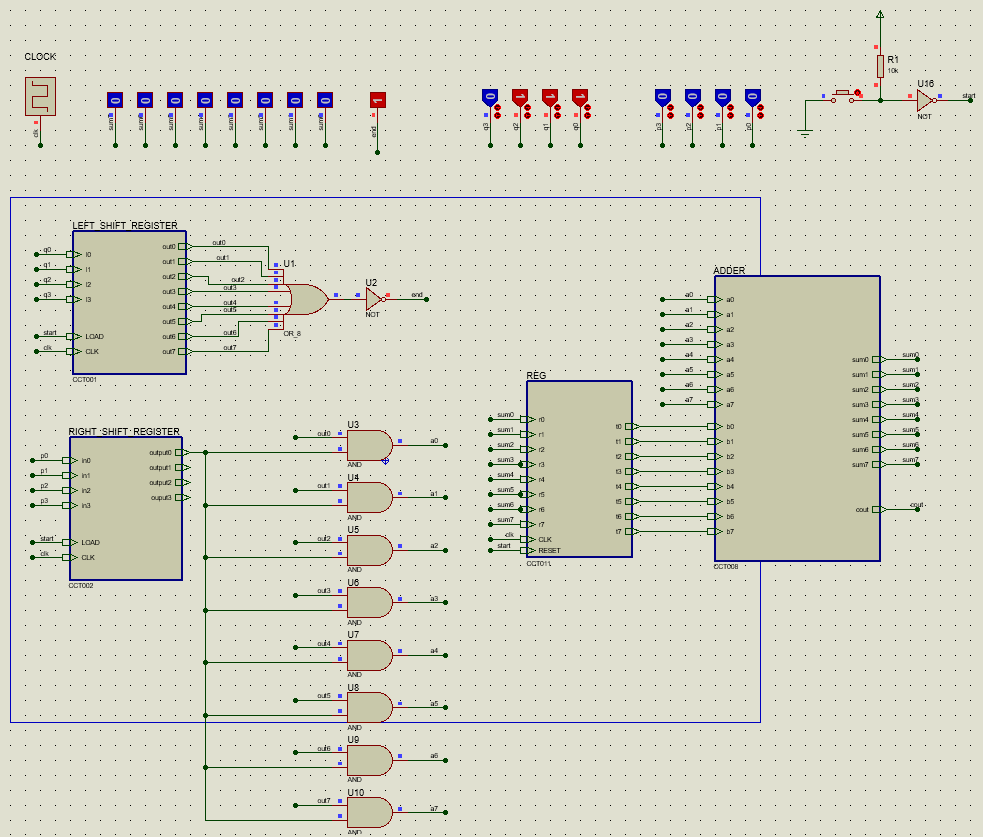
\includegraphics[width=0.8\textwidth]{source/test3.png}
		\caption{$7\times 0 = 0$}
		\vspace*{5mm}
		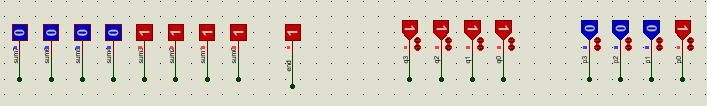
\includegraphics[width=0.8\textwidth]{source/test4.png}
		\caption{$15 \times 1 = 15$}
	\end{figure}
\end{document}







